

%% NJCTL: PSI AP Physics C
%%----------------------------------------


%% Rotational Dynamics
%%----------------------------------------
\element{njctl}{
\begin{question}{rotational-dynamics-q01}
    Torque is the rotational analogue of:
    \begin{choices}
        \wrongchoice{kinetic energy}
        \wrongchoice{linear momentum}
        \wrongchoice{acceleration}
      \correctchoice{force}
        \wrongchoice{mass}
    \end{choices}
\end{question}
}

\newcommand{\njctlRotationDynamicsQTwo}{
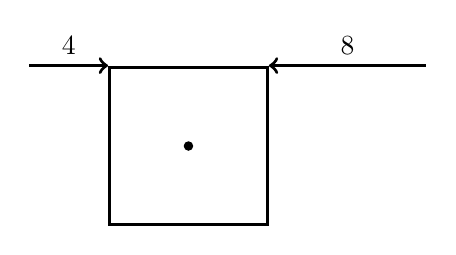
\begin{tikzpicture}
    \draw[fill] (0,0) circle (1.5pt);
    \node[draw,very thick,minimum size=2cm,anchor=center] (B) at (0,0) {};
    \draw[very thick,<-] (B.north west) -- ++(180:1) node[pos=0.5,anchor=south] {\SI{4}{\newton}};
    \draw[very thick,<-] (B.north east) -- ++(0:2) node[pos=0.5,anchor=south] {\SI{8}{\newton}};
\end{tikzpicture}
}

\element{njctl}{
\begin{question}{rotational-dynamics-q02}
    %% Questions 2-4 tikz
    A wooden square of side length \SI{1}{\meter} is on a horizontal tabletop and is free to rotate about its center axis.
    The square is subject to two forces and rotates.
    \begin{center}
        \njctlRotationDynamicsQTwo
    \end{center}
    %% start question
    Find the net torque of the system.
    \begin{multicols}{3}
    \begin{choices}
      \correctchoice{\SI{2}{\newton\meter}}
        \wrongchoice{\SI{12}{\newton\meter}}
        \wrongchoice{\SI[parse-numbers=false]{4\sqrt{2}}{\newton\meter}}
        \wrongchoice{\SI[parse-numbers=false]{2\sqrt{2}}{\newton\meter}}
        \wrongchoice{\SI[parse-numbers=false]{\sqrt{2}}{\newton\meter}}
    \end{choices}
    \end{multicols}
\end{question}
}

\element{njctl}{
\begin{question}{rotational-dynamics-q03}
    %% Questions 2-4 tikz
    A wooden square of side length \SI{1}{\meter} is on a horizontal tabletop and is free to rotate about its center axis.
    The square is subject to two forces and rotates.
    \begin{center}
        \njctlRotationDynamicsQTwo
    \end{center}
    %% start question
    Where should another \SI{4}{\newton} force be applied to maximize its rotational torque?
    \begin{multicols}{2}
    \begin{choices}
        \AMCboxDimensions{down=-1cm}
        \wrongchoice{
            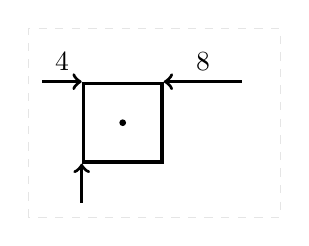
\begin{tikzpicture}
                \draw[white!90!black,dashed] (-1.2,-1.2) rectangle (2,1.2);
                \draw[fill] (0,0) circle (1pt);
                \node[draw,very thick,minimum size=1cm,anchor=center] (B) at (0,0) {};
                \draw[very thick,<-] (B.north west) -- ++(180:0.5) node[pos=0.5,anchor=south] {\SI{4}{\newton}};
                \draw[very thick,<-] (B.north east) -- ++(0:1) node[pos=0.5,anchor=south] {\SI{8}{\newton}};
                \draw[very thick,<-] (B.south west) -- ++(270:0.5) node[pos=0.5,anchor=south] {};
            \end{tikzpicture}
        }
        %% ANS is B
        \correctchoice{
            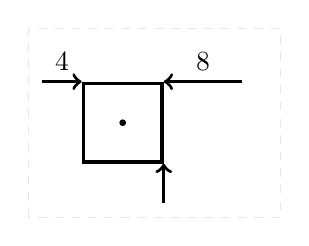
\begin{tikzpicture}
                \draw[white!90!black,dashed] (-1.2,-1.2) rectangle (2,1.2);
                \draw[fill] (0,0) circle (1pt);
                \node[draw,very thick,minimum size=1cm,anchor=center] (B) at (0,0) {};
                \draw[very thick,<-] (B.north west) -- ++(180:0.5) node[pos=0.5,anchor=south] {\SI{4}{\newton}};
                \draw[very thick,<-] (B.north east) -- ++(0:1) node[pos=0.5,anchor=south] {\SI{8}{\newton}};
                \draw[very thick,<-] (B.south east) -- ++(270:0.5) node[pos=0.5,anchor=south] {};
            \end{tikzpicture}
        }
        \wrongchoice{
            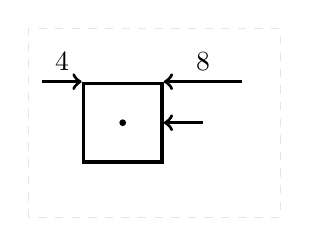
\begin{tikzpicture}
                \draw[white!90!black,dashed] (-1.2,-1.2) rectangle (2,1.2);
                \draw[fill] (0,0) circle (1pt);
                \node[draw,very thick,minimum size=1cm,anchor=center] (B) at (0,0) {};
                \draw[very thick,<-] (B.north west) -- ++(180:0.5) node[pos=0.5,anchor=south] {\SI{4}{\newton}};
                \draw[very thick,<-] (B.north east) -- ++(0:1) node[pos=0.5,anchor=south] {\SI{8}{\newton}};
                \draw[very thick,<-] (B.east) -- ++(0:0.5) node[pos=0.5,anchor=south] {};
            \end{tikzpicture}
        }
        \wrongchoice{
            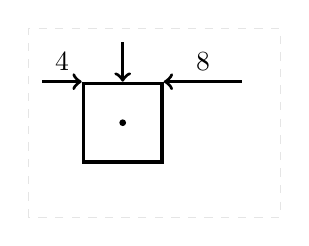
\begin{tikzpicture}
                \draw[white!90!black,dashed] (-1.2,-1.2) rectangle (2,1.2);
                \draw[fill] (0,0) circle (1pt);
                \node[draw,very thick,minimum size=1cm,anchor=center] (B) at (0,0) {};
                \draw[very thick,<-] (B.north west) -- ++(180:0.5) node[pos=0.5,anchor=south] {\SI{4}{\newton}};
                \draw[very thick,<-] (B.north east) -- ++(0:1) node[pos=0.5,anchor=south] {\SI{8}{\newton}};
                \draw[very thick,<-] (B.north) -- ++(90:0.5) node[pos=0.5,anchor=south] {};
            \end{tikzpicture}
        }
        \wrongchoice{
            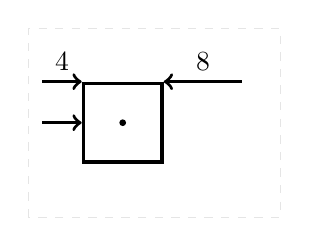
\begin{tikzpicture}
                \draw[white!90!black,dashed] (-1.2,-1.2) rectangle (2,1.2);
                \draw[fill] (0,0) circle (1pt);
                \node[draw,very thick,minimum size=1cm,anchor=center] (B) at (0,0) {};
                \draw[very thick,<-] (B.north west) -- ++(180:0.5) node[pos=0.5,anchor=south] {\SI{4}{\newton}};
                \draw[very thick,<-] (B.north east) -- ++(0:1) node[pos=0.5,anchor=south] {\SI{8}{\newton}};
                \draw[very thick,<-] (B.west) -- ++(180:0.5) node[pos=0.5,anchor=south] {};
            \end{tikzpicture}
        }
    \end{choices}
    \end{multicols}
\end{question}
}

\element{njctl}{
\begin{question}{rotational-dynamics-q04}
    %% Questions 2-4 tikz
    A wooden square of side length \SI{1}{\meter} is on a horizontal tabletop and is free to rotate about its center axis.
    The square is subject to two forces and rotates.
    \begin{center}
        \njctlRotationDynamicsQTwo
    \end{center}
    %% start question
    Where should another \SI{4}{\newton} force be applied to set the wooden square to equilibrium?
    \begin{multicols}{2}
    \begin{choices}
        \AMCboxDimensions{down=-1cm}
        %% ANS is A
        \correctchoice{
            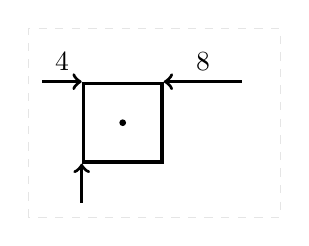
\begin{tikzpicture}
                \draw[white!90!black,dashed] (-1.2,-1.2) rectangle (2,1.2);
                \draw[fill] (0,0) circle (1pt);
                \node[draw,very thick,minimum size=1cm,anchor=center] (B) at (0,0) {};
                \draw[very thick,<-] (B.north west) -- ++(180:0.5) node[pos=0.5,anchor=south] {\SI{4}{\newton}};
                \draw[very thick,<-] (B.north east) -- ++(0:1) node[pos=0.5,anchor=south] {\SI{8}{\newton}};
                \draw[very thick,<-] (B.south west) -- ++(270:0.5) node[pos=0.5,anchor=south] {};
            \end{tikzpicture}
        }
        \wrongchoice{
            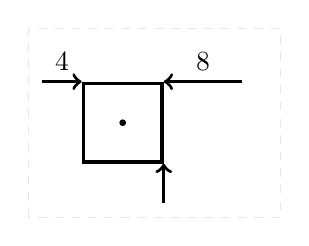
\begin{tikzpicture}
                \draw[white!90!black,dashed] (-1.2,-1.2) rectangle (2,1.2);
                \draw[fill] (0,0) circle (1pt);
                \node[draw,very thick,minimum size=1cm,anchor=center] (B) at (0,0) {};
                \draw[very thick,<-] (B.north west) -- ++(180:0.5) node[pos=0.5,anchor=south] {\SI{4}{\newton}};
                \draw[very thick,<-] (B.north east) -- ++(0:1) node[pos=0.5,anchor=south] {\SI{8}{\newton}};
                \draw[very thick,<-] (B.south east) -- ++(270:0.5) node[pos=0.5,anchor=south] {};
            \end{tikzpicture}
        }
        \wrongchoice{
            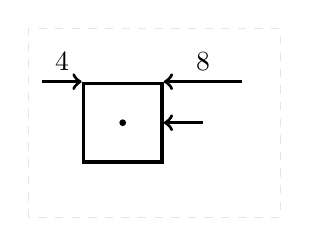
\begin{tikzpicture}
                \draw[white!90!black,dashed] (-1.2,-1.2) rectangle (2,1.2);
                \draw[fill] (0,0) circle (1pt);
                \node[draw,very thick,minimum size=1cm,anchor=center] (B) at (0,0) {};
                \draw[very thick,<-] (B.north west) -- ++(180:0.5) node[pos=0.5,anchor=south] {\SI{4}{\newton}};
                \draw[very thick,<-] (B.north east) -- ++(0:1) node[pos=0.5,anchor=south] {\SI{8}{\newton}};
                \draw[very thick,<-] (B.east) -- ++(0:0.5) node[pos=0.5,anchor=south] {};
            \end{tikzpicture}
        }
        \wrongchoice{
            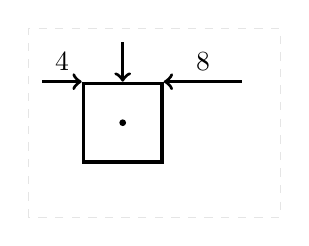
\begin{tikzpicture}
                \draw[white!90!black,dashed] (-1.2,-1.2) rectangle (2,1.2);
                \draw[fill] (0,0) circle (1pt);
                \node[draw,very thick,minimum size=1cm,anchor=center] (B) at (0,0) {};
                \draw[very thick,<-] (B.north west) -- ++(180:0.5) node[pos=0.5,anchor=south] {\SI{4}{\newton}};
                \draw[very thick,<-] (B.north east) -- ++(0:1) node[pos=0.5,anchor=south] {\SI{8}{\newton}};
                \draw[very thick,<-] (B.north) -- ++(90:0.5) node[pos=0.5,anchor=south] {};
            \end{tikzpicture}
        }
        \wrongchoice{
            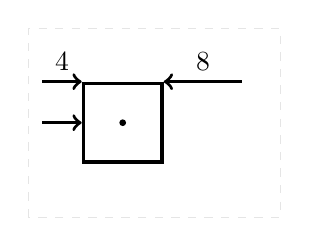
\begin{tikzpicture}
                \draw[white!90!black,dashed] (-1.2,-1.2) rectangle (2,1.2);
                \draw[fill] (0,0) circle (1pt);
                \node[draw,very thick,minimum size=1cm,anchor=center] (B) at (0,0) {};
                \draw[very thick,<-] (B.north west) -- ++(180:0.5) node[pos=0.5,anchor=south] {\SI{4}{\newton}};
                \draw[very thick,<-] (B.north east) -- ++(0:1) node[pos=0.5,anchor=south] {\SI{8}{\newton}};
                \draw[very thick,<-] (B.west) -- ++(180:0.5) node[pos=0.5,anchor=south] {};
            \end{tikzpicture}
        }
    \end{choices}
    \end{multicols}
\end{question}
}

\element{njctl}{
\begin{question}{rotational-dynamics-q05}
    Two wheels are fixed to each other and are free to rotate about a frictionless axis through their concentric center.
    Four forces are exerted tangent to the wheels.
    \begin{center}
    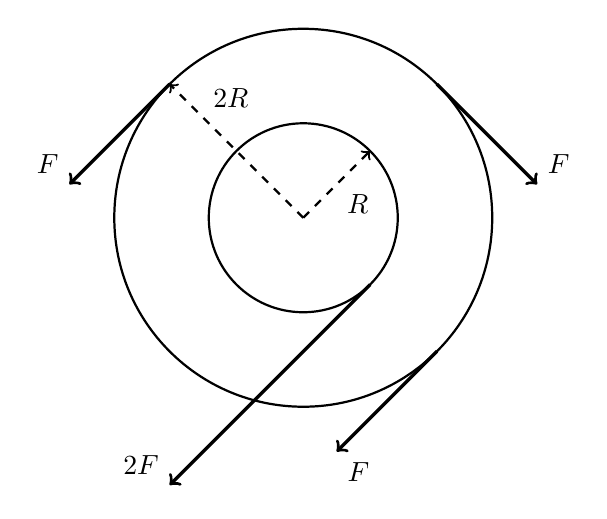
\begin{tikzpicture}[scale=1.2]
        %% Radius
        \draw[thick,dashed,->] (0,0) -- (135:2) node[pos=0.75,anchor=south west] {$2R$};
        \draw[thick,dashed,->] (0,0) -- (45:1) node[pos=0.5,anchor=north west] {$R$};
        %% 2R
        \draw[thick] (0,0) circle (2cm);
        \draw[very thick,->] (135:2) -- ++(225:1.5) node[anchor=south east] {$F$};
        \draw[very thick,->] (45:2) -- ++(315:1.5) node[anchor=south west] {$F$};
        \draw[very thick,->] (315:2) -- ++(225:1.5) node[anchor=north west] {$F$};
        %% 1R
        \draw[thick] (0,0) circle (1cm);
        \draw[very thick,->] (315:1) -- ++(225:3) node[anchor=south east] {$2F$};
    \end{tikzpicture}
    \end{center}
    The magnitude of the net torque is:
    \begin{multicols}{3}
    \begin{choices}
        \wrongchoice{zero}
        \wrongchoice{$FR$}
        \wrongchoice{$2FR$}
      \correctchoice{$4FR$}
        \wrongchoice{$8FR$}
    \end{choices}
    \end{multicols}
\end{question}
}

\element{njctl}{
\begin{question}{rotational-dynamics-q06}
    A baseball player swings his bat with his arms fully extended.
    If his arms are pulled in closer to the body, and he swings again,
        which of the following is true about the angular momentum and kinetic energy of the player?
    \begin{choices}
        %% ANS is C
        \wrongchoice{Angular Momentum increases, Kinetic Energy increases.}
        \wrongchoice{Angular Momentum increases, Kinetic Energy remains constant.}
      \correctchoice{Angular Momentum remains constant, Kinetic Energy increases.}
        \wrongchoice{Angular Momentum remains constant, Kinetic Energy remains constant.}
        \wrongchoice{Angular Momentum decreases, Kinetic Energy remains constant.}
    \end{choices}
\end{question}
}

\element{njctl}{
\begin{question}{rotational-dynamics-q07}
    A tire of mass $M$ and radius $R$ rolls on a flat track without slipping.
    If the angular velocity of the wheel is $\omega$,
        what is its linear momentum?
    \begin{multicols}{2}
    \begin{choices}
      \correctchoice{$M\omega R$}
        \wrongchoice{$M\omega^2 R$}
        \wrongchoice{$M\omega R^2$}
        \wrongchoice{$\dfrac{M\omega^2 R^2}{2}$}
        \wrongchoice{zero}
    \end{choices}
    \end{multicols}
\end{question}
}

\element{njctl}{
\begin{question}{rotational-dynamics-q08}
    A toy car drives around a circular track with a radius of \SI{10}{\meter}.
    When the car's velocity is instantaneously directed south,
        its acceleration is directed west at \SI{10}{\meter\per\second\squared}.
    When viewed from above, the car moves:
    \begin{choices}
      \correctchoice{clockwise at \SI{1}{\radian\per\second}}
        \wrongchoice{clockwise at \SI{10}{\radian\per\second}}
        \wrongchoice{counterclockwise at \SI{1}{\radian\per\second}}
        \wrongchoice{counterclockwise at \SI{10}{\radian\per\second}}
        \wrongchoice{with constant velocity}
    \end{choices}
\end{question}
}

\element{njctl}{
\begin{question}{rotational-dynamics-q09}
    Two masses, one with mass $m$ and the other with mass $2m$,
        are attached to a light rigid rod as shown below.
    \begin{center}
    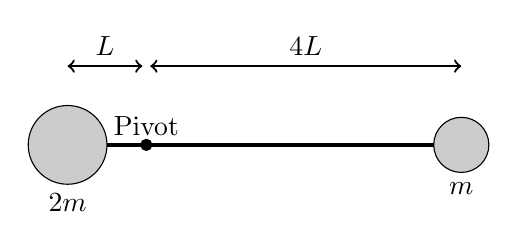
\begin{tikzpicture}
        %% Connection
        \draw[ultra thick] (-1.0,0) --(4,0);
        \draw[fill] (0,0) circle (2pt) node[pos=0.5,anchor=south] {Pivot};
        %% left mass
        \draw[fill=white!80!black] (-1,0) circle (0.5cm) node[anchor=north,yshift=-0.5cm] {$2m$};
        %% right mass
        \draw[fill=white!80!black] (4,0) circle (0.35cm) node[anchor=north,yshift=-0.35cm] {$m$};
        %% length
        \draw[thick,<->] (-1,1) -- (-0.05,1) node[pos=0.5,anchor=south] {$L$};
        \draw[thick,<->] (0.05,1) -- (4,1) node[pos=0.5,anchor=south] {$4L$};
    \end{tikzpicture}
    \end{center}
    When the system is released from rest,
        the rod begins to rotate with an angular acceleration magnitude of:
    \begin{multicols}{3}
    \begin{choices}
        \wrongchoice{$\dfrac{g}{7L}$}
        \wrongchoice{$\dfrac{g}{5L}$}
        \wrongchoice{$\dfrac{g}{4L}$}
        \wrongchoice{$\dfrac{5g}{7L}$}
      \correctchoice{$\dfrac{g}{9L}$}
    \end{choices}
    \end{multicols}
\end{question}
}

\element{njctl}{
\begin{question}{rotational-dynamics-q10}
    A rubber band ball of mass $M$ and radius $R$
        (moment of inertia $\dfrac{2}{5}MR^2$) rolls without slipping up an incline with an initial speed $v$.
    The ball reaches a maximum vertical height of:
    \begin{multicols}{3}
    \begin{choices}
        \wrongchoice{$\dfrac{v^2}{5g}$}
        \wrongchoice{$\dfrac{2v^2}{5g}$}
        \wrongchoice{$\dfrac{v^2}{2g}$}
      \correctchoice{$\dfrac{7v^2}{10g}$}
        \wrongchoice{$\dfrac{v^2}{g}$}
    \end{choices}
    \end{multicols}
\end{question}
}

\element{njctl}{
\begin{question}{rotational-dynamics-q11}
    A dart of mass $m$ moves with a constant speed $v_0$ along the dashed line.
    The dart strikes a uniform disk of radius $R$.
    \begin{center}
    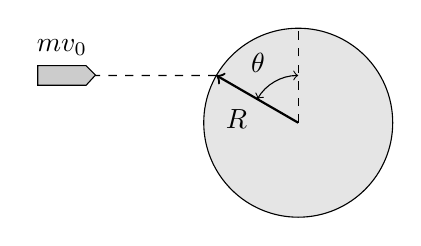
\begin{tikzpicture}[scale=1.2]
        %% uniform disk
        \draw[fill=white!90!black] (0,0) circle ( );
        \draw[thick,->] (0,0) -- (150:1) node[pos=0.5,anchor=north east] {$R$};
        \draw[dashed] (0,0) -- (90:1);
        \draw[<->] (150:0.5) arc(150:90:0.5) node[pos=0.5,anchor=south east] {$\theta$};
        %% rocket
        \node[anchor=center,minimum width=0.6cm,minimum height=0.1cm] (R) at (-2.5,0.5) {};
        \draw[dashed] (150:1) -- (R.east);
        \draw[fill=white!80!black] (R.north west) -- (R.north east) -- ++(-45:0.14) -- (R.south east) -- (R.south west) -- cycle;
        \node[anchor=south] at (R.north) {$mv_0$};
    \end{tikzpicture}
    \end{center}
    What is the magnitude of the angular momentum of the dart with respect to the center of the disk?
    \begin{multicols}{2}
    \begin{choices}
        \wrongchoice{zero}
        \wrongchoice{$mv_0 R\sin\theta$}
        \wrongchoice{$mv_0 R$}
      \correctchoice{$mv_0 R\cos\theta$}
        \wrongchoice{$mv_0$}
    \end{choices}
    \end{multicols}
\end{question}
}

\element{njctl}{
\begin{question}{rotational-dynamics-q12}
    %% Questions 12-13
    A wheel with rotational inertia $I$ is placed on an axle and is free to rotate without friction.
    The angular speed $\omega$ of the wheel is increased from zero to $\omega_f$ in a time interval $t$.
    %% start question
    What is the average net torque on the wheel during this time interval?
    \begin{multicols}{3}
    \begin{choices}
        \wrongchoice{$\dfrac{\omega_f}{t}$}
        \wrongchoice{$\dfrac{\omega_f}{t^2}$}
        \wrongchoice{$\dfrac{I\omega_f^2}{t}$}
        \wrongchoice{$\dfrac{I\omega_f}{t^2}$}
      \correctchoice{$\dfrac{I\omega_f}{t}$}
    \end{choices}
    \end{multicols}
\end{question}
}

\element{njctl}{
\begin{question}{rotational-dynamics-q13}
    %% Questions 12-13
    A wheel with rotational inertia $I$ is placed on an axle and is free to rotate without friction.
    The angular speed $\omega$ of the wheel is increased from zero to $\omega_f$ in a time interval $t$.
    %% start question
    What is the average power input to the wheel during this time interval?
    \begin{multicols}{3}
    \begin{choices}
        \wrongchoice{$\dfrac{I\omega_f}{2t}$}
      \correctchoice{$\dfrac{I\omega_f^2}{2t}$}
        \wrongchoice{$\dfrac{I\omega_f^2}{2t^2}$}
        \wrongchoice{$\dfrac{I^2\omega_f}{2t^2}$}
        \wrongchoice{$\dfrac{I^2\omega_f^2}{2t^2}$}
    \end{choices}
    \end{multicols}
\end{question}
}

\element{njctl}{
\begin{questionmult}{rotational-dynamics-q14}
    A satellite of mass $m$ moves with a constant speed $v$ in a circular orbit of radius $r$.
    \begin{center}
    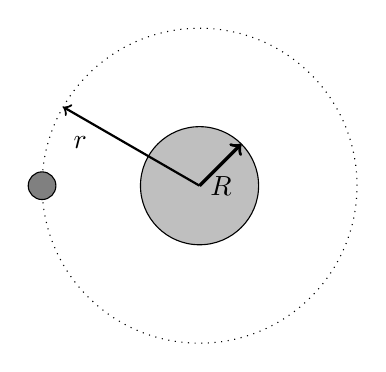
\begin{tikzpicture}
        %% planet
        \draw[fill=white!75!black] (0,0) circle (0.75cm);
        \draw[very thick,->] (0,0) -- (45:0.75) node[pos=0,anchor=west] {$R$};
        %% orbit
        \draw[dotted] (0,0) circle (2cm);
        \draw[thick,->] (0,0) -- (150:2) node[pos=0.75,anchor=north east] {$r$};
        %% satellite
        \draw[fill=white!50!black] (-2,0) circle (5pt);
    \end{tikzpicture}
    \end{center}
    Which of the following statements are true?
    \begin{choices}
      \correctchoice{Its angular speed is $\dfrac{v}{r}$.}
      \correctchoice{Its tangential acceleration is zero.}
      \correctchoice{The magnitude of its centripetal acceleration is constant.}
        %\wrongchoice{I only}
        %\wrongchoice{II only}
        %\wrongchoice{I and III only}
        %\wrongchoice{II and III only}
        %\correctgchoice{I, II, and III}
    \end{choices}
\end{questionmult}
}

\element{njctl}{
\begin{question}{rotational-dynamics-q15}
    A planet moves in an elliptical orbit around the Sun.
    \begin{center}
    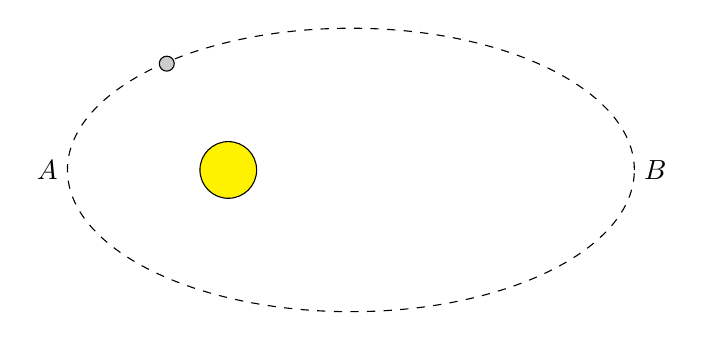
\begin{tikzpicture}[scale=0.9]
        %% Planet and orbit
        \draw[dashed] (0,0) circle (4cm and 2cm);
        %% Planet and satellite
        \draw[fill=yellow] (-1.73,0) circle (0.4cm) node[anchor=south,yshift=0.4cm] {};
        \draw[fill=white!80!black] (150:3) circle (3pt) node[anchor=south east] {};
        %% A and B
        \node[anchor=east] at (-4,0) {$A$};
        \node[anchor=west] at (+4,0) {$B$};
    \end{tikzpicture}
    \end{center}
    As it moves from point $A$ to point $B$,
        which of the following is true about its speed and angular momentum?
    \begin{choices}
        %% ANS is E
        \wrongchoice{Speed remains constant, Angular Momentum remains constat.}
        \wrongchoice{Speed increases, Angular Momentum increases.}
        \wrongchoice{Speed decreases, Angular Momentum decreases.}
        \wrongchoice{Speed increases, Angular Momentum remains constant.}
      \correctchoice{Speed decreases, Angular Momentum remains constant.}
    \end{choices}
\end{question}
}

%\element{njctl}{
%\begin{question}{rotational-dynamics-q16}
%    In which of the following diagrams is the torque about point $C$ equal in magnitude to the torque about point $C$ in the diagram above?
%    All forces lie in the plane of the paper.
%    %\begin{multicols}{2}
%    \begin{choices}
%        \AMCboxDimensions{down=-0.5cm}
%        %% NOTE: ANS is E
%        %% TODO: draw tikz
%        \wrongchoice{
%            \begin{tikzpicture}
%                \draw[dashed] (-3,-1) rectangle (3,1);
%                \node[anchor=north east] at (-2,-0.1) {$C$};
%                \draw (-2,-0.1) rectangle (2,0.1);
%                \draw[dashed,->] (-2,0.5) -- (2,0.5) node[pos=0.5,anchor=south] {$L$};
%                \draw[very thick,->] (+2,-0.1) -- ++(240:1) node[pos=0.8,anchor=north west] {$2F$};
%            \end{tikzpicture}
%        }
%    \end{choices}
%    %\end{multicols}
%\end{question}
%}
%
%\newcommand{\njctlRotationalDynamicsQSeventeen}{
%\begin{tikzpicture}
%    %% TODO: draw tikz
%    %% long cylinder
%    \draw (0,0,3) circle (0.2cm);
%    %% fat center
%    \draw[fill=white!50!black] (0,0,-0.2) circle (1.5cm);
%    \draw[fill=white] (0,0,+0.2) circle (1.5cm);
%    \draw[thick,->] (3,0,0) -- (1.5,0,0) node[pos=0.5,anchor=east] {4};
%    \draw (0,0,3) circle (0.2cm);
%\end{tikzpicture}
%}
%
%\element{njctl}{
%\begin{question}{rotational-dynamics-q17}
%    %% Questions 17-18
%    A clay blob of mass $m$ is stuck to a wheel of radius $R$ rotates clockwise with constant angular velocity $\omega$.
%    The clay mass passes through points 1, 2, 3, and 4 before making a full revolution.
%    \begin{center}
%        \njctlRotationalDynamicsQSeventeen
%    \end{center}
%    %% start question
%    At which point will the net force on the mass be greatest?
%    \begin{multicols}{2}
%    \begin{choices}
%        \wrongchoice{Point 1}
%        \wrongchoice{Point 2}
%        \wrongchoice{Point 3}
%        \wrongchoice{Point 4}
%      \correctchoice{At all points the net force is the same}
%    \end{choices}
%    \end{multicols}
%\end{question}
%}
%
%\element{njctl}{
%\begin{question}{rotational-dynamics-q18}
%    %% Questions 17-18
%    A clay blob of mass $m$ is stuck to a wheel of radius $R$ rotates clockwise with constant angular velocity $\omega$.
%    The clay mass passes through points 1, 2, 3, and 4 before making a full revolution.
%    \begin{center}
%        \njctlRotationalDynamicsQSeventeen
%    \end{center}
%    %% start question
%    What is the minimum adhesive force necessary for the clay to stay attached to the wheel at point 3?
%    \begin{multicols}{2}
%    \begin{choices}
%        \wrongchoice{$mg$}
%        \wrongchoice{$m\omega^2 R$}
%        \wrongchoice{$m\omega^2 R^2 + mg$}
%        \wrongchoice{$m\omega^2 R - mg$}
%      \correctchoice{$m\omega^2 R + mg$}
%    \end{choices}
%    \end{multicols}
%\end{question}
%}

\newcommand{\njctlRotationalDynamicsQNineteen}{
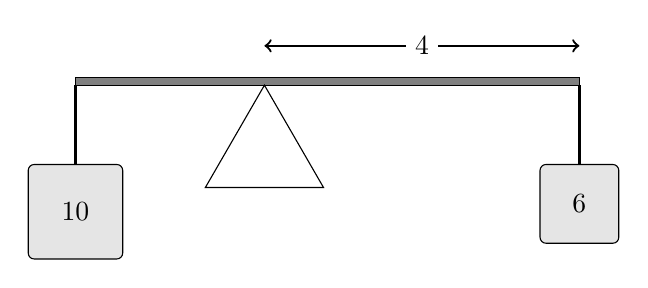
\begin{tikzpicture}
    %% NOTE:
    %% Rod
    \draw[fill=white!50!black] (-2.4,0) rectangle (4,0.1);
    %% pivot
    \draw (0,0) -- ++(300:1.5) -- ++(180:1.5) -- cycle;
    %% masses
    \node[draw,minimum size=1.2cm,rounded corners=0.5ex,fill=white!90!black,anchor=north] (L) at (-2.4,-1) {\SI{10}{\kilo\gram}};
    \node[draw,minimum size=1.0cm,rounded corners=0.5ex,fill=white!90!black,anchor=north] (R) at (+4.0,-1) {\SI{6}{\kilo\gram}};
    \draw[thick] (L.north) -- (-2.4,0);
    \draw[thick] (R.north) -- (+4.0,0);
    %% distance label
    \draw[<->,thick] (0,0.5) -- (4,0.5) node[pos=0.5,anchor=center,fill=white] {\SI{4}{\meter}};
\end{tikzpicture}
}

\element{njctl}{
\begin{question}{rotational-dynamics-q19}
    %% Questions 19-20
    Two masses of mass \SI{10.0}{\kilo\gram} and \SI{6.0}{\kilo\gram} are hung from massless strings at the end of a light rod.
    The rod itself is virtually weightless.
    A pivot is placed off center and the system is free to rotate.
    \begin{center}
        \njctlRotationalDynamicsQNineteen
    \end{center}
    %% start question
    If the rod is at equilibrium (not rotating) and the \SI{6}{\kilo\gram} mass is \SI{4}{\meter} away from the pivot how far away is the \SI{10}{\kilo\gram} mass?
    \begin{multicols}{2}
    \begin{choices}
        \wrongchoice{\SI{0.42}{\meter}}
      \correctchoice{\SI{2.4}{\meter}}
        \wrongchoice{\SI{4.8}{\meter}}
        \wrongchoice{\SI{6.3}{\meter}}
        \wrongchoice{\SI{9.8}{\meter}}
    \end{choices}
    \end{multicols}
\end{question}
}

\element{njctl}{
\begin{question}{rotational-dynamics-q20}
    %% Questions 19-20
    Two masses of mass \SI{10.0}{\kilo\gram} and \SI{6.0}{\kilo\gram} are hung from massless strings at the end of a light rod.
    The rod itself is virtually weightless.
    A pivot is placed off center and the system is free to rotate.
    \begin{center}
        \njctlRotationalDynamicsQNineteen
    \end{center}
    %% start question
    The string supporting \SI{6}{\kilo\gram} block is cut.
    Find the magnitude of the net torque of the system.
    \begin{multicols}{3}
    \begin{choices}
        \wrongchoice{\SI{60}{\newton\meter}}
        \wrongchoice{\SI{120}{\newton\meter}}
      \correctchoice{\SI{240}{\newton\meter}}
        \wrongchoice{\SI{480}{\newton\meter}}
        \wrongchoice{zero}
    \end{choices}
    \end{multicols}
\end{question}
}

\element{njctl}{
\begin{question}{rotational-dynamics-q21}
    Which of the following must be true for the below system to be at equilibrium?
    \begin{center}
    \begin{tikzpicture}[font=\small]
        %% Ceiling
        \node[anchor=south,fill,pattern=north east lines,minimum width=3cm, minimum height=0.05cm] at (0,0) {};
        \draw (-1.5,0) -- (1.5,0);
        %% Masses
        \node[draw,fill=white!90!black,rectangle,rounded corners=1ex,minimum size=1.00cm] (A) at (-1.00,-3) {$m_2$};
        \node[draw,fill=white!90!black,rectangle,rounded corners=1ex,minimum size=1.22cm] (B) at (+0.50,-4) {$m_1$};
        %% Pulley
        \draw[thick] (0,-1.25) circle (1.00);
        \draw[thick] (0,-1.25) circle (0.50);
        \draw[fill=white!50!black] (-0.25,0) -- (-0.15,-1.3) arc(190:350:0.15) -- (0.25,0) --cycle;
        \draw[fill] (0,-1.25) circle (1.5pt);
        \draw[thick,->] (0,-1.25) -- ++(160:1) node[anchor=east] {$R_2$};
        \draw[thick,->] (0,-1.25) -- ++(20:0.5) node[anchor=west] {$R_1$};
        %% Rope
        \draw[thick] (A.north) -- (-1.00,-1.25);
        \draw[thick] (B.north) -- (+0.50,-1.25);
    \end{tikzpicture}
    \end{center}
    \begin{multicols}{2}
    \begin{choices}
        \wrongchoice{$m_1 = m_2$}
      \correctchoice{$R_1 m_1 = R_2 m_2$}
        \wrongchoice{$R_1 m_2 = R^2 m_1$}
        \wrongchoice{$R_1^2 m_1 = R_2^2 m_2$}
        \wrongchoice{$R_2^2 m_1 = R_1^2 m_2$}
    \end{choices}
    \end{multicols}
\end{question}
}

\newcommand{\njctlRotationDynamicsQTwentyTwo}{
\begin{tikzpicture}
    %% Ground
    \node[anchor=north,fill,pattern=north east lines,minimum width=8cm, minimum height=0.05cm] at (0,0) {};
    \draw (-4,0) -- (4,0);
    %% incline
    \draw[thick] (3,0) -- (-3,3.46) -- (-3,0) -- cycle;
    %% height
    \draw[<->] (-3.5,0) -- (-3.5,3.46) node[pos=0.5,anchor=center,fill=white] {$H$};
    %% angle
    \draw[<->] (1,0) arc(180:150:2) node[pos=0.5,anchor=east] {$\theta$};
    %% ball
    \draw[shading=ball,ball color=white!80!black] (3,0) ++ (150:6) arc(240:-120:0.33);
\end{tikzpicture}
}

\element{njctl}{
\begin{question}{rotational-dynamics-q22}
    A ball of rotational inertia $\dfrac{2}{5}MR^2$ is released from rest at the top of an incline of height $H$ at an angle $\theta$.
    There is no friction between the ball and the surface of the incline.
    \begin{center}
        \njctlRotationDynamicsQTwentyTwo
    \end{center}
    What is the acceleration of the ball as it slides down the incline?
    \begin{multicols}{2}
    \begin{choices}
        \wrongchoice{$\dfrac{g}{2}$}
      \correctchoice{$g\sin\theta$}
        \wrongchoice{$2g\cos\theta$}
        \wrongchoice{$g\sin^2\theta$}
        \wrongchoice{zero}
    \end{choices}
    \end{multicols}
\end{question}
}

\element{njctl}{
\begin{question}{rotational-dynamics-q23}
    A ball of rotational inertia $\dfrac{2}{5}MR^2$ is released from rest at the top of an incline of height $H$ at an angle $\theta$.
    There is no friction between the ball and the surface of the incline.
    \begin{center}
        \njctlRotationDynamicsQTwentyTwo
    \end{center}
    How fast does the ball travel at the bottom of the incline?
    \begin{multicols}{2}
    \begin{choices}
        \wrongchoice{$2gH$}
        \wrongchoice{$gH$}
        \wrongchoice{$4gH \sin\theta$}
      \correctchoice{$\sqrt{2gH}$}
        \wrongchoice{$\sqrt{\dfrac{H}{g}}$}
    \end{choices}
    \end{multicols}
\end{question}
}

\element{njctl}{
\begin{question}{rotational-dynamics-q24}
    %% NOTE: TODO: This should be reworded, remove in another scenario to make independent
    A ball of rotational inertia $\dfrac{2}{5}MR^2$ is released from rest at the top of an incline of height $H$ at an angle $\theta$.
    There is no friction between the ball and the surface of the incline.
    \begin{center}
        \njctlRotationDynamicsQTwentyTwo
    \end{center}
    In another scenario there is friction between the ball and incline so that the ball rolls down without slipping.
    %% start question
    How fast does the ball travel at the bottom of the incline?
    \begin{multicols}{2}
    \begin{choices}
        \wrongchoice{$2gH$}
        \wrongchoice{$gH$}
      \correctchoice{$\sqrt{\dfrac{10gH}{7}}$}
        \wrongchoice{$\sqrt{2gH}$}
        \wrongchoice{$\sqrt{\dfrac{H}{g}}$}
    \end{choices}
    \end{multicols}
\end{question}
}

\element{njctl}{
\begin{question}{rotational-dynamics-q25}
    %% NOTE: TODO: This should be reworded, remove in another scenario to make independent
    A ball of rotational inertia $\dfrac{2}{5}MR^2$ is released from rest at the top of an incline of height $H$ at an angle $\theta$.
    There is no friction between the ball and the surface of the incline.
    \begin{center}
        \njctlRotationDynamicsQTwentyTwo
    \end{center}
    In another scenario there is friction between the ball and incline so that the ball rolls down without slipping.
    %% start question
    What is the acceleration of the ball as it rolls down the incline?
    \begin{multicols}{2}
    \begin{choices}
        \wrongchoice{$\dfrac{g}{2}$}
        \wrongchoice{$g\sin\theta$}
        \wrongchoice{$\mu mg\cos\theta$}
        \wrongchoice{$mg\sin^2\theta$}
      \correctchoice{$\dfrac{5g\sin\theta}{7}$}
    \end{choices}
    \end{multicols}
\end{question}
}

\element{njctl}{
\begin{question}{rotational-dynamics-q26}
    %% NOTE: TODO: This should be reworded, remove in another scenario to make independent
    A ball of rotational inertia $\dfrac{2}{5}MR^2$ is released from rest at the top of an incline of height $H$ at an angle $\theta$.
    There is no friction between the ball and the surface of the incline.
    \begin{center}
        \njctlRotationDynamicsQTwentyTwo
    \end{center}
    In another scenario there is friction between the ball and incline so that the ball rolls down without slipping.
    %% start question
    Which of the following is true about the energy of the ball as it rolls down the inclined?
    \begin{choices}
        \wrongchoice{Initial potential energy is equally divided between translational and rotational kinetic energies}
        \wrongchoice{The rotational kinetic energy is always greater than translational kinetic energy}
        \wrongchoice{The translational kinetic energy is zero when the ball rolls down the inclined}
        \wrongchoice{The amount of the rotational kinetic energy gained by the ball depends on its mass}
      \correctchoice{The amount of the rotational kinetic energy gained by the ball depends on its moment of inertia}
    \end{choices}
\end{question}
}

\element{njctl}{
\begin{question}{rotational-dynamics-q27}
    Three objects of the same mass and radius are released at the top of an inclined plane:
        a disk with moment of inertia $\dfrac{1}{2}MR^2$,
        a hoop with moment of inertia $MR^2$ and a sphere with moment of inertia $\dfrac{2}{5}MR^2$.
    How will the speed at the bottom of the incline be different for all three objects as they roll down without slipping?
    \begin{choices}
        \wrongchoice{The disk will travel faster}
        \wrongchoice{The hoop will travel faster}
      \correctchoice{The sphere will travel faster}
        \wrongchoice{They have the same speed at the bottom of the inclined}
        \wrongchoice{None of the provided}
    \end{choices}
\end{question}
}

\newcommand{\njctlRotationDynamicsQTwentyEight}{
\begin{tikzpicture}
    %% NOTE:
    %% Rod of length L
    \draw (-3,0) rectangle (3,0.2);
    %% Center of mass
    \draw[fill] (0,0.1) circle (1.5pt);
    %% labels
    \draw[<->,dashed] (-3,0.75) -- (3,0.75) node[pos=0.5,anchor=center,fill=white] {$L$};
    \draw[<->,dashed] (-3,-0.50) -- (-1.5,-0.50) node[pos=0.5,anchor=center,fill=white] {$L/4$};
\end{tikzpicture}
}

\element{njctl}{
\begin{question}{rotational-dynamics-q28}
    %% Questions 28-29
    A rod of length $L$ is rotated about its center,
        which has a moment of inertia $\dfrac{1}{12}ML^2$.
    \begin{center}
        \njctlRotationDynamicsQTwentyEight
    \end{center}
    What is the moment of inertia at a point $\dfrac{L}{4}$ away from the center?
    \begin{multicols}{3}
    \begin{choices}
        \wrongchoice{$\dfrac{1}{12} ML^2$}
        \wrongchoice{$\dfrac{3}{4} ML^2$}
      \correctchoice{$\dfrac{7}{48} ML^2$}
        \wrongchoice{$\dfrac{15}{29} ML^2$}
        \wrongchoice{$ML^2$}
    \end{choices}
    \end{multicols}
\end{question}
}

\element{njctl}{
\begin{question}{rotational-dynamics-q29}
    %% Questions 28-29
    A rod of length $L$ is rotated about its center,
        which has a moment of inertia $\dfrac{1}{12}ML^2$.
    \begin{center}
        \njctlRotationDynamicsQTwentyEight
    \end{center}
    What is the moment of inertial with respect to the end of the rod?
    \begin{multicols}{3}
    \begin{choices}
        \wrongchoice{$\dfrac{1}{12} ML^2$}
      \correctchoice{$\dfrac{1}{3} ML^2$}
        \wrongchoice{$\dfrac{7}{12} ML^2$}
        \wrongchoice{$\dfrac{1}{6} ML^2$}
        \wrongchoice{$\dfrac{19}{26} ML^2$}
    \end{choices}
    \end{multicols}
\end{question}
}

\element{njctl}{
\begin{question}{rotational-dynamics-q30}
    The system below rotates with an angular velocity $\omega$.
    \begin{center}
    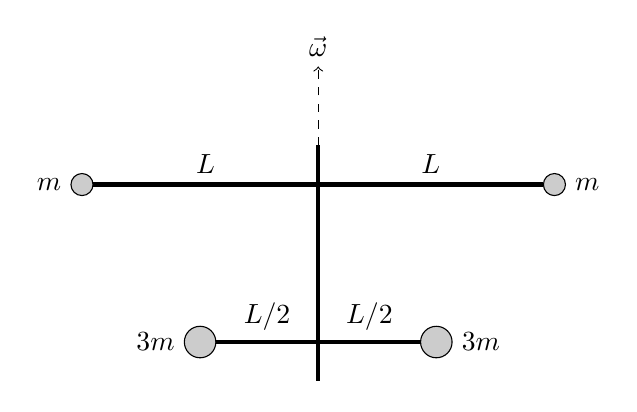
\begin{tikzpicture}
        %% vertical bar
        \draw[ultra thick] (0,1.5) -- (0,-1.5);
        \draw[dashed,->] (0,1.5) -- (0,2.5) node[anchor=south] {$\vec{\omega}$};
        %% mass m, length L
        \draw[fill=white!80!black] (-3,1) circle (0.14cm) node[anchor=east,xshift=-0.14cm] {$m$};
        \draw[fill=white!80!black] (+3,1) circle (0.14cm) node[anchor=west,xshift=+0.14cm] {$m$};
        \draw[ultra thick] (-2.86,1) -- (+2.86,1)
            node[pos=0.25,anchor=south] {$L$}
            node[pos=0.75,anchor=south] {$L$};
        %% mass 3m, length L/2
        \draw[fill=white!80!black] (-1.5,-1) circle (0.2cm) node[anchor=east,xshift=-0.2cm] {$3m$};
        \draw[fill=white!80!black] (+1.5,-1) circle (0.2cm) node[anchor=west,xshift=+0.2cm] {$3m$};
        \draw[ultra thick] (-1.3,-1) -- (+1.3,-1)
            node[pos=0.25,anchor=south] {$L/2$}
            node[pos=0.75,anchor=south] {$L/2$};
    \end{tikzpicture}
    \end{center}
    If the masses of the rod supports are negligible,
        what is the ratio of the angular momentum of the two upper spheres to the angular momentum of the two lower spheres?
    \begin{multicols}{3}
    \begin{choices}
        %% ratios or fractions??
        \wrongchoice{$\dfrac{2}{1}$}
      \correctchoice{$\dfrac{4}{3}$}
        \wrongchoice{$\dfrac{3}{4}$}
        \wrongchoice{$\dfrac{1}{4}$}
        \wrongchoice{$\dfrac{1}{1}$}
    \end{choices}
    \end{multicols}
\end{question}
}

\element{njctl}{
\begin{question}{rotational-dynamics-q31}
    The moment of inertia of a cylinder of mass $M$ and radius $R$ is $\dfrac{1}{2} MR^2$ when the axis of rotation passes through its center.
    \begin{center}
    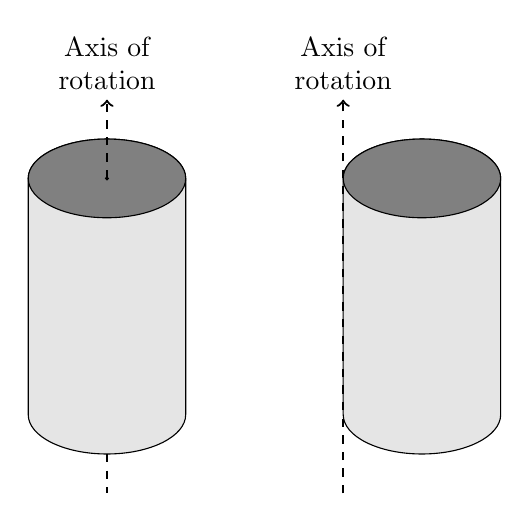
\begin{tikzpicture}
        \begin{scope}[xshift=-2cm]
            \draw[fill=white!90!black] (-1,0) arc (180:0:1cm and 0.5cm) -- (1,-3) arc(0:-180:1cm and 0.5cm) -- (-1,0) --cycle;
            \draw[fill=white!50!black] (-1,0) arc(180:-180:1cm and 0.5cm);
            \draw[fill] (0,0) circle (0.5pt);
            \draw[thick,dashed] (0,-3.5) -- (0,-4);
            \draw[thick,dashed,->] (0,0) -- (0,1) node[anchor=south,text width=5em,text centered] {Axis of rotation};
        \end{scope}
        \begin{scope}[xshift=+2cm]
            \draw[fill=white!90!black] (-1,0) arc (180:0:1cm and 0.5cm) -- (1,-3) arc(0:-180:1cm and 0.5cm) -- (-1,0) --cycle;
            \draw[fill=white!50!black] (-1,0) arc(180:-180:1cm and 0.5cm);
            %\draw[fill] (0,0) circle (1.5pt);
            \draw[thick,dashed,->] (-1,-4) -- (-1,1) node[anchor=south,text width=5em,text centered] {Axis of rotation};
        \end{scope}
    \end{tikzpicture}
    \end{center}
    The moment of inertia of the cylinder about the axis of rotation tangent to the cylinder is:
    \begin{multicols}{3}
    \begin{choices}
        \wrongchoice{$\dfrac{1}{2} MR^2$}
        \wrongchoice{$\dfrac{1}{4} MR^2$}
      \correctchoice{$\dfrac{3}{4} MR^2$}
        \wrongchoice{$\dfrac{3}{2} MR^2$}
        \wrongchoice{$\dfrac{5}{2} MR^2$}
    \end{choices}
    \end{multicols}
\end{question}
}

\element{njctl}{
\begin{question}{rotational-dynamics-q32}
    A uniform beam of length $L$ and mass $m$ is mounted by a hinge on a wall.
    The beam is held in a horizontal position by a wire that makes an angle $\theta$ with the horizontal.
    \begin{center}
    \begin{tikzpicture}
        %% Wall
        \node[anchor=east,fill,pattern=north east lines,minimum width=0.05cm, minimum height=5cm] at (0,1.5) {};
        \draw (0,-1) -- (0,4);
        %% Rod
        \draw[fill] (0,-0.5) -- (0,0.05) arc (90:-90:0.05) --cycle;
        \draw (0,0.1) arc (90:-90:0.1);
        \draw[fill=white!90!black] (0.1,-0.1) rectangle (5,0.1);
        \node[anchor=south] at (2,0.1) {$m$};
        %% Wire
        \draw[thick] (5,0.1) -- (0,3) node[pos=0.5,anchor=south] {$T$};
        \draw[<->] (3.5,0.1) arc(180:149:1.5) node[pos=0.5,anchor=east] {$\theta$};
    \end{tikzpicture}
    \end{center}
    Which of the following is equal to the tension force $T$ in the wire?
    \begin{multicols}{3}
    \begin{choices}
        \wrongchoice{$\dfrac{mg}{2\cos\theta}$}
      \correctchoice{$\dfrac{mg}{2\sin\theta}$}
        \wrongchoice{$\dfrac{mg}{2\tan\theta}$}
        \wrongchoice{$\dfrac{mg}{\cos\theta}$}
        \wrongchoice{$\dfrac{mg}{\sin\theta}$}
    \end{choices}
    \end{multicols}
\end{question}
}

\element{njctl}{
\begin{question}{rotational-dynamics-q33}
    A disk is free to rotate about an axis perpendicular to the disk and passing through its center.
    If the disk starts from rest and accelerates uniformly at the rate of \SI{5}{\radian\per\second\squared} for \SI{4}{\second},
        what its angular displacement during this time?
    \begin{multicols}{3}
    \begin{choices}
        \wrongchoice{\SI{10}{\radian}}
        \wrongchoice{\SI{20}{\radian}}
        \wrongchoice{\SI{30}{\radian}}
      \correctchoice{\SI{40}{\radian}}
        \wrongchoice{\SI{50}{\radian}}
    \end{choices}
    \end{multicols}
\end{question}
}

\element{njctl}{
\begin{question}{rotational-dynamics-q34}
    A circular platform of mass $M$ and radius $R$ rotates about a fixed pivot at its center with an initial angular velocity $\omega$.
    A boy of mass $m$ initially standing at the edge of the platform jumps off the platform with a velocity $v$ with respect to the ground.
    \begin{center}
    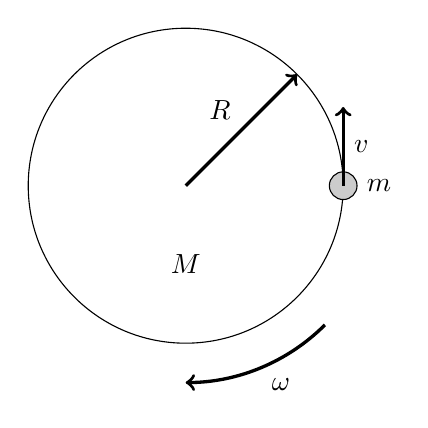
\begin{tikzpicture}
        %% Circular path
        \draw (0,0) circle (2cm);
        %% Mass
        \draw[fill=white!80!black] (0:2) circle (5pt) node[anchor=west,xshift=5pt] {$m$};
        \draw[very thick,->] (0:2) -- ++(90:1) node[pos=0.5,anchor=west] {$v$};
        %% Radius
        \draw[very thick,->] (0,0) -- (45:2) node[pos=0.5,anchor=south east] {$R$};
        %% Mass
        \node[anchor=center] at (270:1) {$M$};
        %% omega
        \draw[very thick,->] (315:2.5) arc (315:270:2.5) node[pos=0.5,anchor=north west] {$\omega$};
    \end{tikzpicture}
    \end{center}
    What is the new angular velocity of the platform?
    \begin{choices}
        \wrongchoice{$\dfrac{\left(M+2m\right)\omega R-2mv}{MR}$}
        \wrongchoice{$\dfrac{\left(M-2m\right)\omega R-2mv}{MR}$}
      \correctchoice{$\dfrac{\left(M+2m\right)\omega R+2mv}{MR}$}
        \wrongchoice{$\dfrac{\left(M+2m\right)\omega R-2mv}{R}$}
        \wrongchoice{$\dfrac{\left(M+2m\right)\omega R-2mv}{M}$}
    \end{choices}
\end{question}
}

\element{njctl}{
\begin{question}{rotational-dynamics-q35}
    A uniform ladder of length $L$ is supported by a person holding end $A$ so the ladder makes an angle $\theta$ with the horizontal.
    There is no friction between the ladder and the floor.
    When the ladder is dropped it falls down because of gravity.
    \begin{center}
    \begin{tikzpicture}
        %% Ground
        \node[anchor=north,fill,pattern=north east lines,minimum width=8cm, minimum height=0.05cm] at (0,0) {};
        \draw (-4,0) -- (4,0);
        %% NOTE: is there suppose to be a frictionless wall?
        %% Wall
        %\node[anchor=north,fill,pattern=north east lines,minimum width=8cm, minimum height=0.05cm] at (0,0) {};
        %\draw (-4,0) -- (4,0);
        %% Ladder length L
        \draw[line width=3pt] (2,0) -- ++(135:5)
            node[pos=1.0,anchor=south east] {$A$}
            node[pos=0.5,anchor=south west] {$L$}
            node[pos=0.0,anchor=south west] {$B$};
        \draw[<->] (0,0) arc (180:135:2) node[pos=0.5,anchor=east] {$\theta$};
    \end{tikzpicture}
    \end{center}
    Which of the following correctly describes the movement of end $B$ as the ladder falls?
    \begin{choices}
        %% NOTE: double check answers
        \wrongchoice{It stays at rest}
        \wrongchoice{It moves a distance $L\sin\theta$ to the right}
      \correctchoice{It moves a distance $L\cos\theta$ to the right}
        \wrongchoice{It moves a distance $L\sin\theta$ to the left}
        \wrongchoice{It moves a distance $L\cos\theta$ to the left}
    \end{choices}
\end{question}
}

\element{njctl}{
\begin{question}{rotational-dynamics-q36}
    A disk with mass $M$ and radius $R$,
        and moment of inertia $I = \dfrac{1}{2} MR^2$ rotates at a constant angular velocity $\omega_0$ about its center.
    \begin{center}
    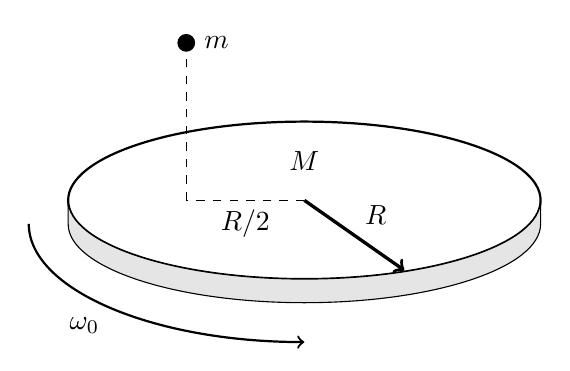
\begin{tikzpicture}
        %% disk
        \draw[thick] (0,0) circle (3cm and 1cm);
        \draw[fill=white!90!black] (-3,0) -- (-3,-0.3) arc(180:360:3cm and 1cm) -- (+3,0) arc(0:-180:3cm and 1cm) --cycle;
        \draw[very thick,->] (0,0) -- (325:1.55) node[pos=0.5,anchor=south west] {$R$};
        \node[anchor=center] at (90:0.5) {$M$};
        %% mass
        \draw[dashed] (0,0) -- (-1.5,0) node[pos=0.5,anchor=north] {$R/2$};
        \draw[dashed] (-1.5,0) -- (-1.5,2);
        \draw[fill] (-1.5,2) circle (3pt) node[anchor=west,xshift=3pt] {$m$};
        %% omega
        \draw[thick,->] (-3.5,-0.3) arc(180:270:3.5cm and 1.5cm) node[pos=0.5,anchor=north east] {$\omega_0$};
    \end{tikzpicture}
    \end{center}
    A piece of clay with mass $m$ is dropped and lands on the surface of the disk at a point $R/2$ from the center of the disk.
    What is the new angular velocity of the disk-clay system?
    \begin{multicols}{3}
    \begin{choices}
        \wrongchoice{$\dfrac{4M\omega_0}{M+\frac{m}{2}}$}
        \wrongchoice{$\dfrac{3M\omega_0}{M+\frac{m}{2}}$}
        \wrongchoice{$\dfrac{5M\omega_0}{M+\frac{m}{2}}$}
      \correctchoice{$\dfrac{M\omega_0}{M+\frac{m}{2}}$}
        \wrongchoice{$\dfrac{9M\omega_0}{M+\frac{m}{2}}$}
    \end{choices}
    \end{multicols}
\end{question}
}

\element{njctl}{
\begin{question}{rotational-dynamics-q37}
    Two disks with radii $R$ and $3R$ are connected by a rubber belt which doesn't slip on the surface of each disk.
    \begin{center}
    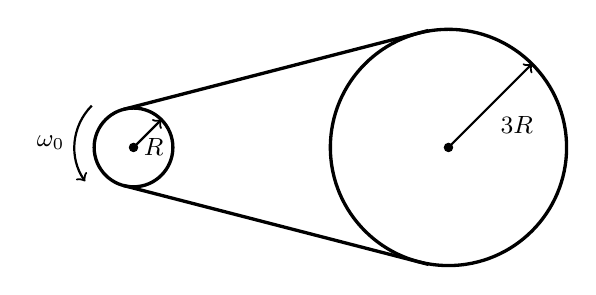
\begin{tikzpicture}[font=\small]
        %% left disk
        \draw[very thick] (-2,0) circle (0.5cm);
        \draw[fill] (-2,0) circle (1.5pt);
        \draw[thick,->] (-2,0) -- ++(45:0.5) node[pos=0,anchor=west] {$R$};
        \draw[thick,->] (-2,0) ++(135:0.75) arc(135:215:0.75) node[pos=0.5,anchor=east] {$\omega_0$};
        %% right disk
        \draw[very thick] (+2,0) circle (1.5cm);
        \draw[fill] (+2,0) circle (1.5pt);
        \draw[thick,->] (+2,0) -- ++(45:1.5) node[pos=0.5,anchor=north west] {$3R$};
        %% Rope
        \draw[very thick] (-2,0) ++(104.5:0.5) -- ++(14.5:4);
        \draw[very thick] (-2,0) ++(-104.5:0.5) -- ++(-14.5:4);
    \end{tikzpicture}
    \end{center}
    If the small disk rotates with an angular velocity $\omega_0$,
        what is the angular velocity of the larger disk?
    \begin{multicols}{3}
    \begin{choices}
        \wrongchoice{$\omega_0$}
        \wrongchoice{$3\omega_0$}
      \correctchoice{$\dfrac{1}{3}\omega_0$}
        \wrongchoice{$\dfrac{2}{3}\omega_0$}
        \wrongchoice{$\dfrac{3}{2}\omega_0$}
    \end{choices}
    \end{multicols}
\end{question}
}

\element{njctl}{
\begin{question}{rotational-dynamics-q38}
    Two blocks with masses $m_1$ and $m_2$ are connected by a light string that passes over a pulley with moment of inertia $I$.
    \begin{center}
    \begin{tikzpicture}[font=\small]
        %% Ceiling
        \node[anchor=south,fill,pattern=north east lines,minimum width=3cm, minimum height=0.05cm] at (0,0) {};
        \draw (-1.5,0) -- (1.5,0);
        %% Masses
        \node[draw,fill=white!90!black,rectangle,rounded corners=1ex,minimum size=1.00cm] (A) at (-0.75,-4) {$m_1$};
        \node[draw,fill=white!90!black,rectangle,rounded corners=1ex,minimum size=1.22cm] (B) at (+0.75,-3) {$m_2$};
        %% Rope
        \draw[thick] (A.north) -- (-0.75,-1) arc(180:0:0.75) -- (B.north);
        %% Pulley
        \draw[thick] (0,-1.00) circle (0.75);
        \draw[fill=white!50!black] (-0.25,0) -- (-0.15,-1.1) arc(190:350:0.15) -- (0.25,0) --cycle;
        \draw[fill] (0,-1.00) circle (1.5pt);
        \draw[thick,->] (0,-1.00) -- ++(20:0.75) node[pos=0.5,anchor=north] {$R$};
        \node[anchor=center] at (-0.50,-1.00) {$I$};
    \end{tikzpicture}
    \end{center}
    If $m_2$ is greater than $m_1$,
        what is the acceleration of the system after it was released from rest?
    \begin{multicols}{2}
    \begin{choices}
        \wrongchoice{$\dfrac{\left(m_2+m_1\right)g}{m_1+m_2+\frac{I}{R^2}}$}
      \correctchoice{$\dfrac{\left(m_2-m_1\right)g}{m_1+m_2+\frac{I}{R^2}}$}
        \wrongchoice{$\dfrac{\left(m_2+m_1\right)g}{m_1+m_2}$}
        \wrongchoice{$\dfrac{\left(m_2+m_2\right)g}{m_1-m_2}$}
        \wrongchoice{$\dfrac{\left(2m_2+m_2\right)g}{m_1+m_2+\frac{I}{R^2}}$}
    \end{choices}
    \end{multicols}
\end{question}
}

\element{njctl}{
\begin{questionmult}{rotational-dynamics-q39}
    A disk slides at a constant speed on the top of a horizontal frictionless table.
    The disk collides with a stationary rod that is pivoted on one end.
    \begin{center}
    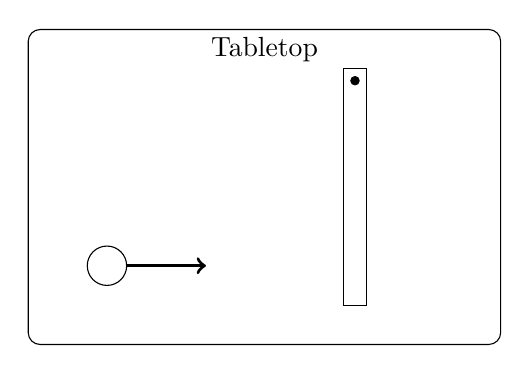
\begin{tikzpicture}
        %% Table
        \draw[rounded corners=1ex] (-3,-2) rectangle (3,2);
        \node[anchor=center] at (0,1.75) {Tabletop};
        %% Ball
        \node[draw,circle,minimum size=0.5cm] (B) at (-2,-1) {};
        \draw[very thick,->] (B.east) -- ++(0:1);
        %% Rod
        \draw (1,-1.5) rectangle (1.30,1.5);
        \draw[fill] (1.15,1.35) circle (1.5pt);
    \end{tikzpicture}
    \end{center}
    Which of the following must be the same for the disk-rod system before and after the collision?
    \begin{choices}
        \wrongchoice{Linear momentum}
      \correctchoice{Angular momentum}
        \wrongchoice{Kinetic energy}
        %\wrongchoice{I only}
        %\correctchoice{II only}
        %\wrongchoice{I and II only}
        %\wrongchoice{I and III only}
        %\wrongchoice{II and III only}
    \end{choices}
\end{questionmult}
}

\element{njctl}{
\begin{question}{rotational-dynamics-q40}
    A uniform ladder of mass $m$ leans without slipping against a smooth wall.
    The coefficient of static friction between the ladder and the floor is $\mu$.
    \begin{center}
    \begin{tikzpicture}
        %% NOTE: should the wall be visible in graphic?
        %% Wall and Floor
        \draw (0,0) -- (5,0);
        \node[anchor=north,fill,pattern=north east lines,minimum width=5.0cm, minimum height=0.05cm] at (2.5,0) {};
        \draw (0,0) -- (0,5);
        \node[anchor=east,fill,pattern=north east lines,minimum width=0.05cm, minimum height=5.2cm] at (0,2.4) {};
        %% ladder
        \draw[ultra thick] (0,4) -- (4,0);
        %% angle
        \draw[<->] (2.5,0) arc(180:135:1.5) node[pos=0.5,anchor=east] {$\theta$};
    \end{tikzpicture}
    \end{center}
    The minimum value of angle $\theta$ that can prevent the ladder from sliding on the floor is:
    \begin{multicols}{2}
    \begin{choices}
      \correctchoice{$\tan^{-1}\left(\dfrac{1}{2\mu}\right)$}
        \wrongchoice{$\sin^{-1}\left(\dfrac{1}{2\mu}\right)$}
        \wrongchoice{$\cos^{-1}\left(\dfrac{1}{2\mu}\right)$}
        \wrongchoice{$\cot^{-1}\left(\dfrac{1}{2\mu}\right)$}
        \wrongchoice{$\dfrac{1}{2\mu}$}
    \end{choices}
    \end{multicols}
\end{question}
}


%% Answers:
%% 1.D 2.A 3.B 4.A 5.D 6.C 7.A 8.A 9.E 10.D 11.D 12.E 13.B 14.E 15. E 16.E 17.E 18.E 19.B 20.C 21.B 22.B 23.D 24.C 25.E 26.E 27.C 28.C 29.B 30.B 31.C 32.B 33.D 34.C 35.C 36.D 37.C 38.B 39.B 40.A


\endinput


